\documentclass[tikz, border=0.15mm]{standalone}
\usepackage{ytableau,tikz,varwidth}
\usetikzlibrary{calc}
\usepackage{mathrsfs}
\newcommand{\typeA}{magenta!65}
\newcommand{\typeB}{blue!75}
\newcommand{\typeC}{green!65}

\begin{document}
\ytableausetup{mathmode, boxframe=normal, boxsize=2.5em}
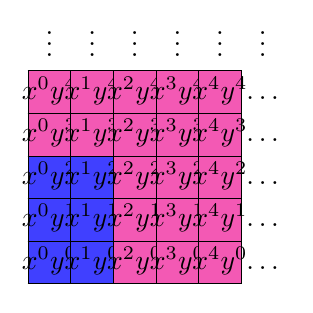
\begin{tikzpicture}[inner sep=0in,outer sep=0in]
	\node (n) {\begin{varwidth}{10cm}{
				\begin{ytableau}
					\none[\vdots] & \none[\vdots] & \none[\vdots] & \none[\vdots] & \none[\vdots] & \none[\vdots] \\
					*(\typeA) x^0y^4 & *(\typeA) x^1y^4 & *(\typeA) x^2y^4 & *(\typeA) x^3y^4 & *(\typeA) x^4y^4 & \none[\dots] \\
					*(\typeA) x^0y^3 & *(\typeA) x^1y^3 & *(\typeA) x^2y^3 & *(\typeA) x^3y^3 & *(\typeA) x^4y^3 & \none[\dots] \\
					*(\typeB) x^0y^2 & *(\typeB) x^1y^2 & *(\typeA) x^2y^2 & *(\typeA) x^3y^2 & *(\typeA) x^4y^2 & \none[\dots] \\
					*(\typeB) x^0y^1 & *(\typeB) x^1y^1 & *(\typeA) x^2y^1 & *(\typeA) x^3y^1 & *(\typeA) x^4y^1 & \none[\dots] \\
					*(\typeB) x^0y^0 & *(\typeB) x^1y^0 & *(\typeA) x^2y^0 & *(\typeA) x^3y^0 & *(\typeA) x^4y^0 & \none[\dots] \\
			\end{ytableau}}\end{varwidth}};
	%\draw[thick, black, -stealth] (n.south west)--([xshift=0.4cm]n.south east);
	%\node[xshift = 0.60cm] at (n.south east) {$\mathscr{T}_1$};
	
	%\draw[thick, black, -stealth] (n.south west)--([yshift=0.4cm]n.north west);
	%\node[yshift = 0.55cm] at (n.north west) {$\mathscr{T}_2$};
\end{tikzpicture}
\end{document}